\documentclass[natbib]{svjour3}

% UTF8 support
\usepackage[utf8x]{inputenc}

\usepackage[english]{babel}


\usepackage{graphicx}
\graphicspath{{figs/}}

\usepackage{booktabs}
\usepackage{array}

\usepackage{amsmath}

\usepackage{tikz}
\usetikzlibrary{shapes}

\usepackage{hyperref}
\usepackage{subcaption}

\usepackage[draft, footnote, margin=false]{fixme}

\usepackage{xspace}
\newcommand{\ie}{i.e.\xspace}
\newcommand{\cf}{{\textit{cf}\xspace}}
\newcommand{\eg}{e.g.\xspace}
\newcommand{\al}{{\textit{et al.}\xspace}}

\newcommand{\A}{A\xspace}
\newcommand{\B}{B\xspace}
\newcommand{\C}{C\xspace}

\newcommand{\M}[3]{{\mathcal{M}(#1, #2, #3)}}
\newcommand{\model}[3]{{$\mathcal{M}(#1, #2, #3)$}}
% generic mutual model (gmodel) 
\newcommand{\gmodel}[2]{{$\mathcal{M}(#1, #2)$}}
\newcommand{\Gmodel}[2]{{\mathcal{M}(#1, #2)}}
\newcommand{\refmodel}[2]{{$\mathcal{M}(#1, #2)$}}
\newcommand{\Model}[3]{{$\mathcal{M}^{\circ}(#1, #2, #3)$}}
\newcommand{\gModel}[2]{{$\mathcal{M}^{\circ}(#1, #2)$}}
\newcommand{\Mdeg}[3]{{\mathcal{M}^{\circ}(#1, #2, #3)}}
\newcommand{\gMdeg}[2]{{\mathcal{M}^{\circ}(#1, #2)}}

\newcommand{\groundingcriterion}{{$\mathcal{M}^{\circ}_{min}$}}
\newcommand{\inigrounding}{{$\mathcal{M}^{\circ}_{t_0}$}}

\newcommand{\concept}[1]{{\small \texttt{#1}}}
\newcommand{\stmt}[1]{{\footnotesize \tt $\langle$ #1\relax$\rangle$}}

\usepackage{mathtools}
\DeclarePairedDelimiter\abs{\lvert}{\rvert}%
\newcommand*\mean[1]{\overline{#1}}

\title{The Symmetry of Partner Modelling}

% ANON
%\author{
%    Pierre Dillenbourg
%    \and
%    Séverin Lemaignan
%    \and
%    Mirweis Sangin
%    \and
%    Nicolas Nova
%    \and
%    Gaëlle Molinari
%}
%\institute{
%    Pierre Dillenbourg, Séverin Lemaignan \at Computer-Human Interaction in Learning and Instruction \\
%    École Polytechnique Fédérale de Lausanne (EPFL) \\ CH-1015 Lausanne, Switzerland \\
%    \email{firstname.lastname@epfl.ch}
%    \and
%    Mirweis Sangin \at Use-able consulting \\ CH-1004 Lausanne, Switzerland\\\email{mirweis@gmail.com}
%    \and
%    Nicolas Nova \at Haute École Arts \& Design de Genève \\ CH-1201 Genève, Switzerland\\\email{nicolas.nova@hesge.ch}
%    \and
%    Gaëlle Molinari \at Distance Learning University Switzerland (Unidistance),
%    CH-3960 Sierre, Switzerland\\\email{gaelle.molinari@unidistance.ch}
%}
\author{}
\begin{document}
\maketitle

\begin{abstract}

Collaborative learning has often been associated to the construction of  a
shared   understanding of the situation at hand. The psycholinguistics
mechanisms at work while establishing common grounds are the object of
scientific controversy. We postulate that collaborative tasks require some
level of mutual modelling, \ie that each partner needs some model of what
the other partners know/want/intend at a given time.  We use the term ``some
model'' to stress the fact that this model is not necessarily detailed or
complete, but that we acquire some representations of the persons we
interact with. The question we address is: Does the quality of the partner
model depend upon the modeler's ability to represent his or her partner?
Upon the modelee's ability to make his state clear to the modeler? Or rather upon
the quality of their interactions? We address this question by comparing
the respective accuracies of the models built by different team
members. We therefore report on 5 experiments on collaborative problem solving
or collaborative learning that vary in terms of tasks (how important it is
to build an accurate model) and settings (how difficult it is to build an
accurate model). In 4 studies, the accuracy of the model that \A built about
\B was correlated with the accuracy of the model that \B built about \A,  which
seems to imply that the quality of interactions matters more than individual
abilities when building mutual models.  However, these finding do not
rule out the fact that individual abilities also participate in the quality of
modelling process.


\end{abstract}

\keywords{Cognitive Modelling; Grounding; Theory of Mind}

\section{Introduction}


From its inception, Computer Supported Collaborative Learning (CSCL)
research has been following the suggestion by \citet{roschelle1995construction}
that collaborative learning has something to do with the process of constructing
and maintaining a \emph{shared understanding} of the task at hand. Building a
shared/mutual understanding refers to the upper class of collaborative learning
situations, those in which students should build upon each other's understanding
to refine their own understanding: what is expected to produce learning is not
the mere fact that two students build the same understanding but the cognitive
effort they have to engage to build this shared
understanding~\citep{schwartz1995emergence}. This effort can be observed by the
frequency of rich interactions, \ie interactions whose occurrence has been
related to learning: (self-) explanations in cognitive
science~\citep{chi1989self, webb1991task}, conflict resolution in
socio-cognitive theories~\citep{doise1975social}, mutual
regulation~\citep{blaye1995collaborative} in a Vygostkian perspective, etc. The
construction of a shared understanding has been investigated for several decades
in psycholinguistics, under the  notion of
\emph{grounding}~\citep{clark1986referring}. However, the relevance of grounding
mechanisms for explaining learning outcomes has been questioned in the learning
sciences. Grounding mechanisms are appropriate to explain conversational
events, such as referential failures in short dialogue episodes, but they do hardly
predict deeper phenomena such as \emph{conceptual change} (\ie the acquisition,
acceptation and integration of a new belief into one's mental model) over longer
sessions~\citep{dillenbourg2006sharing}. The cumulative effect of grounding
episodes can probably be better understood from a socio-cultural perspective:

\begin{quote}
Collaborative learning is associated with the increased
cognitive-interactional effort involved in the transition from \emph{learning to
understand each other} to \emph{learning to understand the meanings of the semiotic
tools that constitute the mediators of interpersonal
interaction}~\citep{baker1999role}
\end{quote}

Along this line, several scholars suggest that CSCL research should go deeper in
the understanding of how partners engage into shared meaning
making~\citep{stahl2007meaning} or \emph{intersubjective} meaning
making~\citep{suthers2006technology}.

Paradoxically, while Clark's theory is somewhat too linguistic from a learning
viewpoint, it is criticized at the same time as being too cognitivist by some
psycholinguists, \ie as overestimating the amount of shared knowledge and mutual
representations actually necessary to conduct a dialogue. The fundamental issue,
as old as philosophy, is the degree of coupling between the different levels of
dialogue, mostly between the lexical/syntactical level and the deeper semantic
levels. \citet{pickering2006alignment} argue that mutual understanding
starts mostly with a \emph{superficial alignment} at the level of the linguistic
representations, due to priming mechanisms, and that this local alignment may --
in some cases -- lead to a \emph{global alignment} of the semantic level
(\emph{deep grounding}).  For these authors, the convergence in dialogue, and
even the repair of some misunderstandings, is explained by this mimetic behavior
more than by a monitoring of each other's knowledge: \emph{``...interlocutors do
not need to monitor and develop full common ground as a regular, constant
part of routine conversation, as it would be unnecessary and far too costly.
Establishment of full common ground is, we argue, a specialized and
non-automatic process that is used primarily in times of difficulty (when
radical misalignment becomes apparent).''} (p. 179).  This view is actually not
incompatible with Clark's \emph{grounding
criterion}~\citep{clark1989contributing}: the degree of shared understanding
that peers need to reach depends upon the task they perform. For instance, a
dialogue between two surgeons might rely on superficial alignment if they talk
about their friends but has to guarantee accurate common grounds when talking
about which intervention will be conducted in which way on which patient.  In
this paper, we operationalized the grounding criterion, \ie the necessity for
accurate modelling, as \emph{the correlation between the accuracy of partner models
and measures of team performance}.


This interesting cognitive science debate occurred mostly outside the field of
learning. In education, the question is to relate these mechanisms to learning
outcomes: Is linguistic alignment sufficient to trigger conceptual
change? Does negotiation of meaning only occur when partners monitor
and diagnose each other's knowledge? If the ratio between shallow alignment and
deep grounding depends upon the task, and if deep grounding is a condition for
learning, then the pedagogical challenge is indeed to design tasks that require
deep grounding. Most empirical studies on grounding and alignment are conducted
with simple referencing tasks such as asking the way to the train station
or helping the peer to choose a picture among many. In the studies we report here, we
explore several richer tasks such as arguing on a sensitive issue or building a
concept map.  

Deep grounding or shared meaning making requires some cognitive load. For
\citet{clark1986referring}, what is important is not the individual effort made
by the receiver of a communicative act, but the overall \emph{least collaborative
effort}.  The cost of producing a perfect utterance may be higher than the cost
of repairing the problems that may arise through misunderstandings, and in fact,
subjects tend to make less efforts adapting their utterances to a specific
partner when they know that they can later provide feedback on his/her
%ANON
%understanding~\citep{schober1993spatial}. We introduced the notion of
%\emph{optimal collaborative effort}~\citep{dillenbourg1995evolution} to stress
understanding~\citep{schober1993spatial}. \citet{dillenbourg1995evolution} introduced the notion of
\emph{optimal collaborative effort} to stress
that misunderstanding should not be viewed as something to be avoided (if this
was possible), but as an opportunity to engage into verbalization, explanation,
negotiation, and so forth. This issue is related to the global argument
regarding cognitive load in learning activities, especially in discovery
learning environments: there is no learning without some cognitive load, but
overload may hinder learning~\citep{paas2003cognitive}. In the context of
collaborative learning, we understand the cognitive load induced by mutual
modelling as part of~\citet{schwartz1995emergence} notion of effort towards a
shared understanding. For instance, CSCL researchers expanded the use of
\emph{collaboration scripts}~\citep{kobbe2007specifying}. A script is a pedagogical
method that frames collaborative learning activities in order to foster the
emergence of productive interactions such as argumentation, explanation or
conflict. Conflict-resolution scripts such as the {\sc
ArgueGraph}~\citep{dillenbourg2008mechanics} form pair of students with
opposite opinions, which increases the difficulty of consensus building,
requiring more justifications, more negotiation, more load. Similarly, {\sc
jigsaw} scripts~\citep{aronson1978jigsaw} provide peers with different but
complementary knowledge for augmenting (reasonably) the efforts that group members
have to engage into to reach a shared solution. 

%\paragraph{Theory of Mind}
%
%Theory of Mind (originally defined in~\citep{premack1978does}) is the cognitive
%ability that a subject possesses to represent the mental state of another
%agent, possibly including knowledge that contradicts the subject's own model: for
%example, a book can be at the same time \emph{visible} for myself, and \emph{not
%visible} for you.
%
%Children develop this skill, which is essential to understand others'
%perspectives during interactions, around the age of three. It supposes the
%ability to build, store and retrieve separate models of the knowledge of the
%interactors.
%
%One classical application of this cognitive skill is the so-called
%\emph{False-Belief} experiment (also known as the \emph{Sally and Ann}
%experiment)~\citep{Leslie2000}: a child is asked to watch a scene where two
%people, \A and \B, manipulate objects. Then \A leaves and \B hides away one
%object. When \A comes back, we ask the child ``where do you think \A will
%look for the object?''. Before acquiring a theory of mind, children are not
%able to separate their own (true) model of the world (where they know that
%the object was hidden) from the model of A, which contains \emph{false
%beliefs} on the world (\A still thinks the object is at its original
%position since he did not see \B hiding it).

\vspace{2em}

In summary, the controversy around the cognitive depth of shared understanding
pertains to psycholinguistic, which investigates natural conversations. The
situation is different in collaborative learning; tasks are actually designed
for requiring a deeper negotiation of meaning.  The expertise of CSCL is to design
collaborative situations that create interdependence, avoid group think, and
allows students to detect any ``illusion of shared
understanding''~\citet{cherubini2005grounding}. Our question is hence not
anymore ``do peers build a shared
understanding ?'', but rather ``whenever peers have to build a shared understanding,
how do they achieve it ?''.  This question addresses the mechanisms of grounding, in
which the basic sequence is: make a proposition, detect misunderstanding and, if
any, repair them.  This paper focuses on the middle part, the detection of
misunderstandings.  Detecting a misunderstanding means that the emitter of a
message identifies a mismatch between his communicative intention and the way
his message is understood by his or her partner. Detecting one peer's
misunderstanding is investigated hereafter under the general umbrella of partner
modelling.

 
%These preliminary remarks frame the main question that this article address:
%in order to engage into shared understanding, which is a desirable learning
%situation, do partners have to build a representation of each other's knowledge?
%if so, what exactly is the nature of this mutual modelling? We adopt hereafter a
%constructive approach, first introducing a simple yet convenient model of mutual
%modelling, then analyzing five independent studies in terms of the interactions
%between learning and mutual modelling.





%%%%%%%%%%%%%%%%%%%%%%%%%%%%%%%%%%%%%%%%%%%%%%%%%%%%%%%%%%%%%%%%%%%%%%%%%%%%%%%%%%%%
%%%%%%%%%%%%%%%%%%%%%%%%%%%%%%%%%%%%%%%%%%%%%%%%%%%%%%%%%%%%%%%%%%%%%%%%%%%%%%%%%%%%


\section{Partner Modelling}

We refer to \emph{Partner modelling} as the process of inferring one's partner
mental states. Any claim that students carry out a detailed monitoring of their
peers would be as incorrect as any claim that they do not maintain any
representation at all. If mental modelling had to be permanently detailed and
accurate, subjects would obviously face a huge cognitive load. Conversely, peers
could not collaborate without some minimal amount of mutual modelling.
Collaborative learning dialogue include many instances of utterances such as ``I
thought he would do that'' (first order modelling) or even ``He
thought I would do that but I intended something else.'' (second order
modelling).

%For instance, \A cannot disagree with \B without knowing that \B has a different
%opinion. The mutual model can be \emph{implicit} (\A is not aware of what he knows about
%B), \emph{by-default} (I believe that \B believes what I believe unless contrary
%evidence), \emph{opportunistic} (\A does not model \B unless the conversation requires
%it), \emph{global} (\A infers \B's beliefs based on categories such as age, culture or
%profession) and, of course, it can be incorrect\ldots but it can not remain empty.

The content of the partner model ranges from \emph{dispositional} to
\emph{situational} aspects. The \emph{dispositional} aspects refer to \A's
representation of \B's long term knowledge, skills or traits. It is thus closely
related to the notion of transactive memory~\citep{wegner1987transactive,
moreland1999transactive}.  \emph{Situational} aspects refer to \A's representation of
B's knowledge, behavior or intentions specifically activated in the situation in
which \A and \B are collaborating, some of them being valid for 2 seconds, other
ones for 2 hours. Examples of fragments that constitute \A's model of B
regarding to aspects X, \ie $Model(A,B,X)$, abbreviated \model{A}{B}{X}, could be:

\begin{itemize}

    \item $Model(A,B, knowledge)$: what does \A know about \B's knowledge with
        respect to the task at hand or, inversely, about \B's knowledge gaps?
        When can \A consider \B's statements as reliable? 

    \item $Model(A,B, skills)$: what does \A know about \B's skills with respect to
        the task at hand? May \A expect \B to perform well in a specific subtask?
        The effectiveness of division of labor depends on the quality of this
        mutual model. 

    \item $Model(A,B, goals)$: what does \A know about \B's intentions with respect
        to the project, including \B' motivation and commitment? Can \A trust
        \B
        when \B promises to deliver? 

    \item $Model(A,B, task)$: what does \A know about \B's representation of the
        situation and the task: does \A knows whether \B has the same
        understanding of the problem at stake? 

    \item $Model(A,B, plans)$: what does \A know about \B's strategy. Does A
        understand why \B did what he did? Is \A able to anticipate what \B will do
        next? 

    \item $Model(A,B, ``urgent")$: what does \A know about \B's understanding of \A's
        last utterance: does ``urgent'' means now, soon or ``not too late''?

\end{itemize}

The list of what $X$ stands for in \model{A}{B}{X} is possibly infinite:
beliefs, emotions, history, status, etc. A partner model is likely not a
``box'', \ie not a monolithic representation but rather a mosaic of information
fragments about the partner, with various granularity and various life cycles.
This mosaic is elaborated through a variety of mechanisms, first for building an
initial model of the partner, then for updating this model. As two students meet
for the first time, partners models are initialized by the assumptions they make
upon each other based on cues such as his/her belonging to broad categories
(age, culture, profession, \ldots), stereotypes (sportsmen, junkie, business
women, Swiss,\ldots) as well as physical appearance. Scholars studied how
initial modelling impacts communication. In their experiment,
\citet{slugoski1993attribution} pretended to their subjects that their
(confederate) partner had or had not received the same information. They
observed that the subjects adapted their dialogue by focusing the explanation on
the items that he/she was supposed to ignore.  \citet{brennan1991conversation}
showed that the subjects used different initial strategies in forming queries
depending on who they were told their partner was.  

Initial common grounds are also initiated by co-presence: they include events to
which \A and \B attended together~\citep{clark2002definite} in the physical
space or in their cultural space (\eg ``09-11''). While co-presence means that
they can refer to shared objects and events, it does not imply that they give
them the same meaning. Namely, a shared screen does not mean a shared
understanding~\citep{dillenbourg2006sharing}.

After initialization, partners models are updated during the collaborative work
through verbal and non-verbal interactions. A default inference rule is that ``my
partner agrees with me unless he disagrees'', which rejects the critiques that
partner modelling generates an unbearable cognitive load. This default rule is
superseded by the several mechanisms for monitoring and repairing the partner
understanding: acknowledgement, continuous attention, relevance of next turns,
facial expressions including gaze signals, etc.

Finally, partner modelling does not occur in a vacuum but it is highly
contextualized.  \citet{clark1991grounding} review how the features of the
collaborative situation, namely the media (co-temporality,\ldots), may
facilitate or hamper mutual modelling.  \citet{hutchins1997constructing}
reported a study in which a short silence between two pilots was perfectly
interpreted because it occurred in a highly constrained communication context.
Some environments are more productive than others in helping peers to detect
their misunderstandings.  \citet{roschelle1995construction} reformulate the
design of CSCL interfaces to provide ways for peers to detect and repair their
misunderstanding.




\section{Mutual Modelling}

Mutual modelling is bi-directional. During dyadic problem solving,   partner A
builds some model of \B and \B build some model of \A.  Moreover, these two
processes are not independent: \A's model of what \B knows, include what \B knows
about \A.  This leads to nested levels of  modelling. If \A states ``\B thinks I
am good in maths'', \A builds a \emph{second level} model:
\model{A}{B}{\M{B}{A}{\text{maths-skill}}}. This leads to possibly infinite
regress of nested models: \A saying ``\B knows that I don't expect him to
solve this statistics problem'' corresponds to \\
\model{A}{B}{\M{B}{A}{\M{A}{B}{\text{statistic-skills}}}}.  As we will see in
one study we report on, mutuality also applies to triads in which \A will elaborate
a model of \B and of C, and reciprocally. This is probably also true for larger
groups although one may hypothesize that there exists (yet undefined) group size
from which it is not possible to model all partners individually and, therefore,
members  model  the group as a whole instead as a collection of individuals.  We
do not explore this hypothesis here and limit ourselves to dyads and triads.

This mutuality allows us to address a fundamental question: \emph{does the
quality of partner modelling depend upon the cognitive skills of each partner
(some people being better in perceiving other's states) or does it result from
the quality of interactions among them ?} Behind his question, the reader may
perceive the long lasting debate between tenets of, respectively, the individual
and social views of human cognition.  The simple hypothesis is that when
individual are randomly paired for an experiment, there is no reason for which
their individual cognitive skills would correlate. Therefore, if it occurs that
the quality of the $Model(A,B)$ is correlated with $Model(B,A)$, one may infers
that this quality depends upon what \A and \B have built together while
interacting.

To answer this question, we went back to five previous studies that addressed
various other research questions, but in which the correlation between the
quality of these two models could be computed.  The studies we report do hence
not constitute a clean sequence of experiment to investigate mutual modelling but
the ad-hoc revisiting of previous experiments to explore a question that we had
then neglected. Some of these studies are about collaborative learning while
others are only collaborative problem solving, but the latter rely on rich tasks
that are similar to those we use in CSCL.

\section{A notation for discussing mutual modelling }

Natural language becomes cumbersome when describing things such as ``the model
that \A builds about the model that \B builds about A''. Therefore, to define
hypotheses and report on experiments on mutual modelling, we use  the notation
\model{A}{B}{X} to denote ``\A knows that \B knows X''. This  notation is not
proposed as a formal theory of mutual modelling but as useful simplification for
communicating about mutual modelling. This notation does not mean \A has an
explicit, monolithic representation of \B: it must be understood as an
abstraction referring to complex socio-cognitive processes.  As explained in the
previous section, \A can be fragmented, multi-dimensional, etc. This notation
is neither presented as a computational model of mutual modelling, nor as some
universal formalism; its usefulness is internal to this paper.  Besides, we
refer to the \emph{degree of accuracy} of the model as \Model{A}{B}{X}. We
discuss in the next section the methodological difficulty in measuring this
accuracy.

We parametrize and assess the mutual modelling effort through 3 variables:

\begin{enumerate}

    \item Tasks vary a lot with respect to how much they require mutual
        understanding.  The \emph{grounding criterion} -- denoted
        \groundingcriterion -- represents the minimum level of modelling
        accuracy required for a task $T$ to succeed. Qualitatively, if the
        performance on a given task $T$ is correlated to \Model{A}{B}{X}, then
        \model{A}{B}{X} is significant to $T$ success, and the
        grounding criterion of $X$ for $T$
        ($\mathcal{M}^{\circ}_{min}(A,B,X,T)$) is non-zero.

        Under the assumption that the higher the correlation, the more
        critical \model{A}{B}{X} is to $T$, we hereafter use the correlation
        coefficient as an estimate of \groundingcriterion.
        \vspace{1em}

    \item Before any specific grounding action, there is generally a non-null
        probability that $X$ is mutually understood by \A and \B (\eg $X$ is
        part of \A's and \B's cultures, it is manifest to co-present subjects
        or simply there is not much space for misunderstanding or disagreement
        about $X$). We simply could not collaborate without a certain level of
        initial grounds. We note the theoretical accuracy of \emph{initial
        grounds} $\mathcal{M}^{\circ}_{t_0}(A,B,X)$.
        \vspace{1em}

    \item The \emph{cost of grounding} $X$ refers to the physical and cognitive
        effort required to perform a grounding act $\alpha$: a verbal repair
        (\eg rephrasing), a deictic gesture, a physical move to adopt one
        partner's viewpoint, etc. This cost varies according to media
        features~\citep{clark1991grounding}.

\end{enumerate}

Based on these 3 parameters, the probability of making an action $\alpha_{t}$
about content $X$ at time $t$ during task T in order to increase \Model{A}{B}{X}
is the ratio between how much it is needed and how much it
costs~\citep{traum1996miscommunication}:

\begin{equation}\label{eq:probrepair}
    p(\alpha_{t}(X,T) /_{\mathcal{M}^{\circ}_{t+1}(A,B,X)\nearrow}) \simeq
    \frac{\mathcal{M}^{\circ}_{min}(A,B,X,T) -
    \mathcal{M}^{\circ}_{t}(A,B,X)}{cost (\alpha_{t})}
\end{equation}

This formula is presented as a qualitative summary, not as a real equation,
since several parameters are hard to quantify (\eg the cost of a communication
act depends upon the user as well).

We can further clarify the parameters in the context of the experiments we
present hereafter:

\begin{itemize}
    \item \Model{A}{B}{X}: our experiments address different contents that can be
        represented in mutual models:

    \begin{enumerate}

        \item \Model{A}{B}{actions} is about how well \A guesses what action \B has
            performed (study 2) or will perform next (study 1),

        \item \Model{A}{B}{emotion}: how accurately \A perceives \B's emotional state
            (study 3),

        \item \Model{A}{B}{knowledge}: how accurately \A estimates \B's knowledge
            with respect to the material they learn together (study 4 and 5).

    \end{enumerate}
        \vspace{1em}

    \item $\mathcal{M}^{\circ}_{min}(A,B,X,T)$: our studies build upon various
        collaborative tasks: argumentation (study 3), games (study 1 and 2) and
        concept mapping (study 4 and 5). By varying the tasks, we do actually
        vary the grounding criterion. The tasks were all designed to require a reasonably high
        grounding criterion, as they are meant for the participants to have to
        actually build a solution or a representation together.
        \vspace{1em}

    \item $\mathcal{M}^{\circ}_{t0}(A,B,X)$: along the same reasoning, the initial degree
        of common grounds should be rather low (and hence the difference between
        initial and required degrees rather high) in order to make mutual
        modelling effort more observable. Studies 1, 4 and 5 have been conducted
        with teams of students who did not know each other. They came
        nonetheless from the same university (and they hence had some general common
        grounds).  For studies 2 and 3, students knew each other before for
        reasons explained later on. In study 5, we manipulated the initial mutual modelling by
        using a {\sc jigsaw} script.
        \vspace{1em}

    \item $cost(\alpha)$: in all studies but study 4, the cost of  grounding is
        an independent variable. Study 3 uses media richness as independent
        variable, with the hypothesis that modelling emotions is ``cheaper'' with a
        richer medium, \ie  when peers can see each other.  Studies 1,2 and 4
        use awareness tools which, in principle, reduce the cost of mutual modelling, but do
        not eliminate all costs: if the tool provides \A with information about
        what \B does/knows, this additional information may actually increase
        cognitive load. Awareness tools constitute a kind of mutual modelling prosthesis,
        and, like any prosthesis, they may augment mutual modelling (by facilitating it or
        even scaffolding it) or inhibit it (by making it useless).

        While we introduce here formally the cost of grounding $cost(\alpha)$ as
        one relevant variable for the discussion of mutual modelling situations,
        we will not attempt to characterize it beyond these qualitative
        observations in the studies we present hereafter.

\end{itemize}


\section{Methodological Issues}

Since a mental model is not directly observable,  the study of mutual modelling
is methodologically difficult. How can we for instance measure \Model{A}{B}{X}?
We proceed in two steps, first to capture \model{A}{B}{X} and then to estimate
\Model{A}{B}{X}. 

{\bf Capturing \model{A}{B}{X}}: The simplest method is to ask \A what he/she
believes about what \B knows, feels, intends to do, etc.  This raises obvious
methodological concerns since such a question triggers a modelling process
beyond what would naturally occur. To avoid this bias, one can estimate mutual
modelling after task completion. Then, the obvious drawback are memory losses
and post-hoc reconstruction. The first method was used in study 2 and the
second one in the other studies. Another option would be to rely on external
behavioural metrics like eye-tracking: we hypothesise for instance that the
fixation time reflects the efforts engaged by the human to understand, hence,
model, the others. Such an approach has however not been investigated in the
presented studies.

{\bf Estimating \Model{A}{B}{X}}: Once \model{A}{B}{X} is captured, we need to
access the reference model \refmodel{B}{X} to estimate its accuracy.
Since we can only indirectly access it via what \B reports (\ie
\model{B}{B}{X}), accuracy can be estimated in 2 ways:

\begin{itemize}

    \item Subjective accuracy: In study 3, for instance, we compute \Model{A}{B}{X} by
        measuring if \A describes \B's emotions in the same way \B reports
        its emotions ($\M{A}{B}{X} = \M{B}{B}{X}$).

    \item Objective accuracy: In studies 4 and 5, we compute \Model{A}{B}{X} by
        comparing \Model{A}{B}{K} to \B's actual knowledge as it has measured
        by a test.

\end{itemize}

Our method for investigating mutual modelling relies on the observation of the variations of
accuracy that result from variations of external parameters (the variables of
the formula~\ref{eq:probrepair} above): for instance, the accuracy should
go down if we increase the cost of grounding acts, and conversly go up if we increase
the grounding criterion (\ie the necessity to build a shared understanding). One way
to produce these variations relies what CSCW researchers call ``awareness
tools'', \ie functionalities that inform \A about \B's actions that \A can
not directly perceive due to \B working in a different subset of the
virtual space. Different awareness tools are used in the following studies as
methodological levers to experimentally manipulate the mutual modelling
activity.


\section{Hypotheses and questions}

The experiments we report here address mutual modelling across different tasks,
some with dyads, other with triads. They were conducted along 6 years in two
different institutions by different researchers. They used different
independent, intermediate and dependent variables. Nonetheless, we were able to
retroactively address 3 research questions across these studies. 

\paragraph{The symmetry question}

As stated earlier, the fundamental challenge is to determine if mutual modelling
is an individual skill (hypothesis $\mathcal{H}_{1}$ below) or  the emergent
property of social interactions (hypothesis $\mathcal{H}_{3}$).  This question
is empirically translated into the symmetry of mutual modelling
(Fig.~\ref{mm_symmetry}): what is the relationship between \Model{A}{B}{X} and
\Model{B}{A}{X}? A low symmetry would mean that mutual modelling is mainly an
individual attitude/aptitude ($\mathcal{H}_{1}$).  A high correlation might
support $\mathcal{H}_{3}$ since there is a low probability that randomly formed
pairs integrate peers with the same level of mutual modelling skills. However, a
high correlation could also have another explanation, stated in
$\mathcal{H}_{2}$: it could be that \A is good at modelling \B and good at
helping \B to model herself or himself.


\begin{itemize}
    \item $\mathcal{H}_{1}$: $\mathcal{M}^{\circ}(A,B)$ depends upon \A's ability or effort
        to model \B,
    
    \item $\mathcal{H}_{2}$: $\mathcal{M}^{\circ}(A,B)$ depends upon  \B's ability or
        effort to help \A to model him/herself,

    \item $\mathcal{H}_{3}$: $\mathcal{M}^{\circ}(A,B)$ depends upon the quality of
        interactions among \A and \B.

\end{itemize}


$\mathcal{H}_{2}$ relates to second level modelling since \B needs to monitor
\A to see if \A understood him/her ($\mathcal{M}(B,A,\mathcal{M}(A,B))$). We
will see that $\mathcal{H}_{2}$ and $\mathcal{H}_{3}$ are actually difficult to
differentiate.



\begin{figure}[htb]
\centering

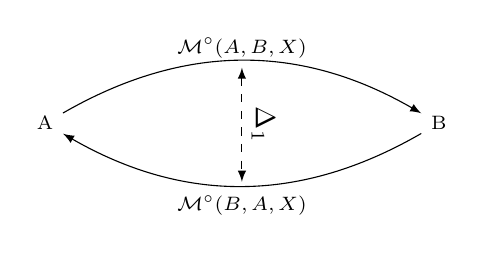
\begin{tikzpicture}[>=latex, scale=0.5]

\draw(0,0) node[anchor=north] (A) {\scriptsize A};
\draw(10,0) node[anchor=north] (B) {\scriptsize B};
\draw(5,2) node[anchor=north] {\scriptsize \Model{A}{ B}{ X}};
\draw(5,-2) node[anchor=north] {\scriptsize \Model{B}{ A}{ X}};
\draw[dashed, <->] (5,1) -- (5,-1.9) node[midway, sloped, above] {$\Delta_1$};
\draw[->] (A) to[bend left] (B);
\draw[->] (B) to[bend left] (A);

\end{tikzpicture}

\caption{\small Mutual modelling in a dyadic interaction, $\Delta_1 =
    \Delta(\mathcal{M}^{\circ} (A,B,X),
\mathcal{M}^{\circ} (B,A,X))$}

\label{mm_symmetry}
\end{figure}

\paragraph{The triangle questions}

With triads, we may compute the accuracy of 6 models: \Model{A}{B}{X},
\Model{B}{A}{X}, \Model{A}{C}{X}, \Model{C}{A}{X}, \Model{C}{B}{X} and
\Model{B}{C}{X}. This leads to two \emph{triangle questions}
(Fig.~\ref{mm_triangles}): Do \A and \B have the same accuracy when modelling
\C ($\Delta_2 = \Delta(\mathcal{M}^{\circ}(A,C,X),
\mathcal{M}^{\circ}(B,C,X))$)? A significant correlation would support ,
$\mathcal{H}_{2}$  (C has helped both \A and \B to model C) or support
$\mathcal{H}_{3}$ (the quality of triad interactions enables all partners to
model each other accurately)  


Conversely, does \C model with similar accuracy \A and \B? (low $\Delta_3=
\Delta(\mathcal{M}^{\circ}(C,A,X), \mathcal{M}^{\circ}(C,B,X))$)? A positive
answer would support $\mathcal{H}_{1}$, \C being simply good at modelling any
partner.  It could also support  $\mathcal{H}_{3}$,  since the quality of
interactions influences the accuracy of two models that \C is building. A
negative answer would support $\mathcal{H}_{2}$ since $\Delta_3$ could mainly be
explained by the fact that  \A helped more \C to model him than \B did. 

In addition, the comparison between $\Delta_2$ and $\Delta_3$ could tell us
whether the accuracy of mutual modelling depends more upon the modeller's effort
($\mathcal{H}_{1}$) or the modellee's behaviour ($\mathcal{H}_{2}$).

Note that we consider the quality of interactions at triad level (\A, \B, \C),
neglecting the cases where \A and \B interact better for instance than \B and \C, since there
was no ``private'' communication channel in the following studies. We do
nonetheless acknowledge that this point could be debated.

\begin{figure}[htb]
\centering
\subcaptionbox{}{ 
    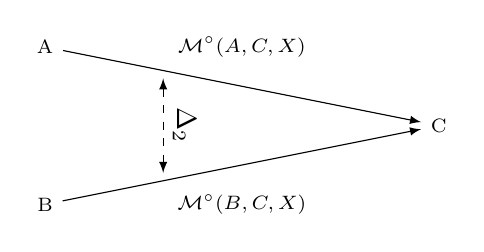
\begin{tikzpicture}[>=latex, scale=0.5]

    \draw(0,2) node (A) {\scriptsize A};
    \draw(0,-2) node (B) {\scriptsize B};
    \draw(10,0) node (C) {\scriptsize C};

    \draw(5,2) node {\scriptsize \Model{A}{ C}{ X}};
    \draw(5,-2) node {\scriptsize \Model{B}{ C}{ X}};
    \draw[dashed, <->] (3,1.2) -- (3,-1.2) node[midway, sloped, above] {$\Delta_2$};
    \draw[->] (A) to (C);
    \draw[->] (B) to (C);

    \end{tikzpicture}
}
\subcaptionbox{}{ 
    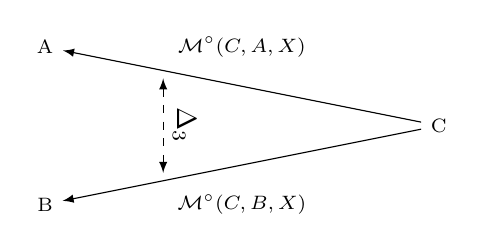
\begin{tikzpicture}[>=latex, scale=0.5]

    \draw(0,2) node (A) {\scriptsize A};
    \draw(0,-2) node (B) {\scriptsize B};
    \draw(10,0) node (C) {\scriptsize C};

    \draw(5,2) node {\scriptsize \Model{C}{ A}{ X}};
    \draw(5,-2) node {\scriptsize \Model{C}{ B}{ X}};
    \draw[dashed, <->] (3,1.2) -- (3,-1.2) node[midway, sloped, above]
    {$\Delta_3$};
    \draw[<-] (A) to (C);
    \draw[<-] (B) to (C);

    \end{tikzpicture}
}
\caption{\small Mutual modelling in a triadic interaction}

\label{mm_triangles}
\end{figure}





\paragraph{The rectangle questions}

We can go further by comparing self- versus other modelling ($\Delta_4$ in
Fig.~\ref{mm_rectangle}). A large difference would indicate that meta-cognitive
skills (self-modelling) and partner modelling skills are rather different
skills, while a small $\Delta_4$ could be interpreted as the indications that
these are two specific instance of a more general cognitive process. This
questions is however not central to this paper, and the value of $\Delta_4$ is
only available in one of the reported studies.

We can also question if modelling skills depend upon what aspects are being
modeled ($X$ or $Y$), which would explain vertical differences ($\Delta_5$ in
Fig.~\ref{mm_rectangle}).  These differences would allow refining the notion of
modelling skills, namely whether there exist some general ability to model
partners or whether this is only the abstraction of a beam of more specific
skills such as detecting emotions versus identifying references from deictic
gestures.

\begin{figure}[htb]
\centering

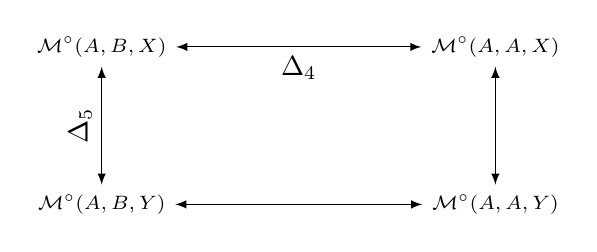
\begin{tikzpicture}[>=latex, scale=0.5]

    \draw(0,0) node (a) {\scriptsize \Model{A}{ B}{ X}};
    \draw(10,0) node (b) {\scriptsize \Model{A}{ A}{ X}};
    \draw(10,-4) node (c) {\scriptsize \Model{A}{ A}{ Y}};
    \draw(0,-4) node (d) {\scriptsize \Model{A}{ B}{ Y}};
    \draw[<->] (a) -- (b) node[midway, below] {$\Delta_4$};
    \draw[<->] (b) -- (c);
    \draw[<->] (c) -- (d);
    \draw[<->] (d) -- (a) node[midway, sloped, above] {$\Delta_5$};

\end{tikzpicture}

\caption{\small Meta-cognitive skills (horizontally) and domain-dependent modelling (vertically}

\label{mm_rectangle}
\end{figure}



%%%%%%%%%%%%%%%%%%%%%%%%%%%%%%%%%%%%%%%%%%%%%%%%%%%%%%%%%%%%%%%%%%%%%%%%%%%%%%%%%%
%%%%%%%%%%%%%%%%%%%%%%%%%%%%%%%%%%%%%%%%%%%%%%%%%%%%%%%%%%%%%%%%%%%%%%%%%%%%%%%%%%



\section{Studies}

We report on five studies conducted  by different researchers in different contexts
between 2000 and 2015. They do not form a consistent research strategy but
actually the fact that some trends emerge despite their diversity constitutes
indeed the richness of this line of work.

\begin{table*}[ht!]
\newcolumntype{L}[1]{>{\raggedright\let\newline\\\arraybackslash\hspace{0pt}}m{#1}}
\centering
%\resizebox{\textwidth}{!}{%
\begin{tabular}{p{2.1cm}L{1.65cm}L{1.7cm}L{1.8cm}L{1.6cm}L{1.6cm}}
\toprule
\textit{}                     & \textbf{Study 1}                 & \textbf{Study 2}                & \textbf{Study 3}          & \textbf{Study 4}          & \textbf{Study 5}             \\ 
\midrule
\textbf{Task}                 & game in virtual space            & game in physical space          & building an argument map  & building a concept map    & building a concept map       \\
\midrule
\textbf{Interactions}         & audio                            & written                         & audio / video             & audio                     & audio                        \\
\midrule
\textbf{Shared editor}        & 3D space                         & 2D map                          & concept map               & concept map               & concept map                  \\
\midrule
\textbf{Group size}           & dyads                            & \textbf{triads}                 & \textbf{triads}           & dyads                     & dyads                            \\
\midrule
\textbf{Duration (mean)}      & 90min                            & 16min                           & 61min                     & 90min                     & 90min                        \\
\midrule
\textbf{Awareness tool}       & partner's position               & partner's current/past pos.     & -                         & partner's concept map     & partner's scores at pre-test \\
\midrule
\textbf{Dependent variable}       & team/indiv. performance            & team/indiv. performance           & team performance          & team/indiv. knowledge       & team/indiv. knowledge          \\
\midrule
\textbf{Independent variable}     & awareness tool \textit{vs} none  & awareness tool \textit{vs} none & audio \textit{vs} audio+video & script \textit{vs} none & awareness tool \textit{vs} none       \\
%\textbf{Grounding crit.}      & +0.42                            & +0.15                           & +0.22                     & +0.08                     & +0.40                        \\
%$\mathcal{H}_1$               &                                  & supported                       & supported                 &                           &                              \\
%$\mathcal{H}_2$               &                                  & supported&                         &                           &                              \\
%$\mathcal{H}_3$               & supported                        & supported                       &                           & supported                 &                              \\
\bottomrule
\end{tabular}
%}
\caption{Overview of the studies}
\label{synthesis_table}
\end{table*}



%%%%%%%%%%%%%%%%%%%%%%%%%%%%%%%%%%%%%%%%%%%%%%%%%%%%%%%%%%%%%%%%%%%%%%%%%%%%%%%%%%
\subsection{{\bf Study 1}: Effect of an awareness tool on \gModel{A}{B} in a virtual
game}

We studied the impact of an awareness tool on group performance and mutual
%ANON
%modelling~\citep{nova2007collaboration}. The availability
modelling \textit{[citation removed for blind review]}. The availability of an
awareness tool was our independent variable. In previous studies, we replayed a
video of the game to subjects who surprised us by their ability to remember
former states of their mutual model: ``I did that because I thought that you
would do that''. Hence, this experiment focused the representation of each
other's action plans. During the game, we asked them to anticipate the next
action of their partner as well as to announce their own actions.

\subsubsection*{Experimental setting}

\begin{figure*}
        \centering
        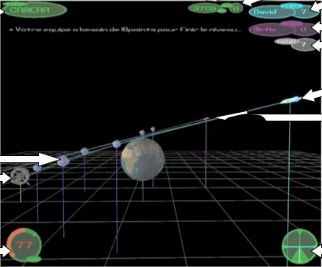
\includegraphics[width=\textwidth]{image4.png}
        \caption{Screenshot of the {\sc SpaceMiners} game}
        \label{study1:spaceminer}
\end{figure*}


{\sc SpaceMiners} is a 3D game that involves two players harvesting ore
found on asteroids (Fig.~\ref{study1:spaceminer}). To do so, they must launch
drones through the space after choosing their initial direction and speed. Once
launched, the trajectory of drones is influenced by the gravity of planets
and by ``trajectory modification'' tools. During the experiment, the teams were
confronted with three increasingly complex situations. The experiment was 2
hours long: a 30 minute tutorial and 3 levels of 30 minutes. The players were using
a regular joystick and communicated with each other through an audio channel.

The independent variable was the availability of an awareness tool that shows to
player \A  the location and gaze direction of player \B: in this ``awareness''
condition, players could switch to the \emph{scout mode} where they could view
what their partner was looking at. We hypothesize that this would enable
subjects to more accurately infer their teammate's intentions. Each player sat
in front of a distinct computer located in different rooms. 

\subsubsection*{Subjects}

Thirty-six persons participated in this study, all native French speakers. We
constituted 18 dyads who did not know each other beforehand. The pairs were
randomly assigned to either the control condition (without the awareness tool)
or the awareness condition (with the awareness tool).

\subsubsection*{Variables}

Task performance was measured by the score reached by the two subjects at the
end of the game (three levels). The effort of mutual modelling was measured as
the ratio of time that players would spend in the scout mode (divided by total
time), which is the time during which players are not performing their own
actions but monitoring their partner's actions.

In order to evaluate \gModel{A}{B} during the task, we used two questionnaires
(Fig.~\ref{study1:questionnaires}) that were displayed during each of the three
games, as a transparent layer appearing over the game display. The first
questionnaire concerned the player's intended actions. The second questionnaire
asked each player about what he thought her or his partner was intending to do.
Some answers were identical in both questionnaires (like ``adjusting a shot'')
while others were reversed (``to guide my partner'' versus ``to guide me'').
This method provides us with a subjective measure of accuracy
($\Delta(\M{A}{A}{X}, \M{A}{B}{X})$) rather than an objective measure (\ie the
model \gmodel{A}{B} is compared to \B's next action) because some of the
activities proposed by the questionnaire were not observable by the environment
(\eg establishing a strategy). We calculated \Model{A}{B}{activity})
as the number of common answers between questionnaires \gmodel{A}{A} and
\gmodel{A}{B} in each game and computed the average value across the 3 levels.

\begin{figure}[ht!]
        \centering
        \includegraphics[width=0.7\columnwidth]{image5.png}
        \caption{\gmodel{A}{A} and \gmodel{A}{B} questionnaires in SpaceMiners
        (translated from French).}

        \label{study1:questionnaires}
\end{figure}

\subsubsection*{Results}

\paragraph{Grounding criterion} The grounding criterion was high: the
correlation between \gModel{A}{B} and task performance was 0.42, $p = 0.05$.
Pairs with an accurate mutual model reached higher scores. A regression analysis
confirmed the positive and significant relation between group performance and
mutual modelling accuracy ($\beta=54, p = 0.02$).

\paragraph{Study-specific questions} The awareness tool permitted higher group
performance, but it did not improve the accuracy of the mutual model. Since
teams were free to use the awareness tool or not (the \emph{scout} mode), we
performed a post-hoc split of players depending on how much time they used it.
The split point was the mean of time spent in the scout mode and it led to the
constitution of two groups made up of 12 individuals ``short time in scout
mode'' and 24 individuals ``long time in scout mode''. A two-way analysis of
variance conducted on these contrasted groups revealed that pairs in the
awareness condition who spent more time in the scout mode reached higher levels
of \gModel{A}{B}($F = 8.02, p = 0.015$). Of course, a post-hoc split
does not support a causal direction. An alternative explanation could be that
good modellers are more social and hence appreciate the awareness tool.

\paragraph{Symmetry question} We computed intra-class correlation as described
by~\citet{kenny1998data} from the answers to the cross-questionnaires.
Considering all pairs in both conditions, we found a positive and significant
correlation ($r = 0.38, p < 0.05$) between \gModel{A}{B} and \gModel{B}{A}.
Interestingly, this was higher in the control group ($r = 0.44$) than in the
experimental group ($r = 0.24$). Actually, $\Delta(\gMdeg{A}{B},\gMdeg{B}{A})$,
\ie the absolute differences between the models accuracy, was not significantly
different with or without the awareness tool ($F [1,13]= 0.144, p > 0.5$). This
result could be explained by the fact that the players without awareness tools
communicated more.

\subsubsection*{The triangle and rectangle questions are not addressed in this study.}

\subsubsection*{Discussion}

How to interpret a correlation of 0.38 between \gModel{A}{B} and \gModel{B}{A}?
It is significant, which supports $\mathcal{H}_{2}$ and $\mathcal{H}_{3}$. It is
nonetheless far from 1 which implies we cannot discard the individual modelling
skills. We collect more evidence along the next studies.

%If it was null, modelling would be interpreted as an individual process that
%varies according to personality traits or cognitive skills: some persons tend to
%model more accurately their peer while others don't care or can simply not
%($\mathcal{H}_{1}$). If the correlation was close to 1, we could conclude that
%the modelling accuracy is an emergent property of teams since there would be low
%probability that, by chance, low accurate modellers are paired with accurate
%modellers and conversely ($\mathcal{H}_{2}$). Our correlation is between these
%two extremes but the very notion of significant intra-class correlation tend to
%indicate that one may not consider peers as independent subjects, which is an
%argument for the \emph{interaction} hypothesis $\mathcal{H}_{3}$. 


%%%%%%%%%%%%%%%%%%%%%%%%%%%%%%%%%%%%%%%%%%%%%%%%%%%%%%%%%%%%%%%%%%%%%%%%%%%%%%%%%%
\subsection{{\bf Study 2}: Effect of an awareness tool on \gModel{A}{B}  in a pervasive
game}

This study concerns a collaborative game that occurred in the physical
%ANON
%space~\citep{nova2006underwhelming}. We studied whether players build an accurate
space \textit{[citation removed for blind review]}. We studied whether players
build an accurate model of the path followed by their partners, assuming that this
path would reflect their problem solving strategy. We used an objective measure of
\gModel{A}{B}: the distance between where \A believes \B has been walking and
where \B actually went.  The main hypothesis concerned the effect of awareness
tools on group performance and on \gModel{A}{B}. 

\subsubsection*{Experimental setting}

{\sc CatchBob} is a mobile game in which groups of 3 players have to solve a
% ANON
%joint task. The game was played on EPFL campus. Participants had to find a
joint task. The game was played on our campus. Participants had to find a
virtual object (\emph{Bob}) and to ``catch'' it by forming a triangle around it.
The players used a Tablet PC that displayed a map of the campus and an indication of
their personal distance to Bob. Their annotations on the map were shared with
the two other players (\A could see what \B and \C wrote). These annotations
faded out after a few minutes to avoid covering the full display. The awareness
tool displayed as well the location of the two other players on the map. Three
conditions were considered: the control condition (without tool) and two
experimental conditions: synchronous awareness (display of the current position
of each player) and asynchronous awareness (display of current position of each
player as well as their recent spatial trace).

\begin{figure*}[h!t] \centering \begin{subfigure}{.45\textwidth}
\includegraphics[width=\linewidth]{image6.png} \caption{A's drawing of \B's
path.} \end{subfigure} \begin{subfigure}{.4\textwidth}
\includegraphics[width=\linewidth]{image7.png} \caption{Actual path followed by
\B.} \end{subfigure} \caption{Reported and actual path of one of the player,
during the {\sc CatchBob} game.} \label{study2:paths} \end{figure*}

\subsubsection*{Subjects}


Ninety students participated in this experiment. We only selected students from
our campus since knowledge of the campus geography had an impact both on group
performance and on mutual modelling: to represent the path of someone across
some space is difficult without an \textit{a priori} mental map of this space.
We formed groups of students who knew each other. We assigned 10 triads to each
of our three experimental conditions. Each condition was made up of
approximately 25\% of women, but we did not control gender repartition within
each triad.

\subsubsection*{Variables}

The independent variable was the presence and role of the awareness tool. As a
dependent variable, we had the task performance which was the distance covered
by the team to catch Bob and \gModel{A}{B}. To estimate \gModel{A}{B}, we asked
players to draw on paper their own path and the path of each of their partners
after the game. This enabled us to calculate the number of errors players made
while drawing the path of their partners. We compared the path that player \A
attributed to \B with \B's real path recorded by the system and the same for \A
\& \C and \B \& \C as depicted on Fig.~\ref{study2:paths}. 

\gModel{A}{B} is the sum of errors made by \A about \B's paths. An error was
either drawing a place where the partner had not been or not drawing a place
where he/she had gone. One could argue that \gModel{A}{B} is biased by the
subjects' ability to translate the memory of their trajectories into a map drawing.
However, 85\% of subjects made no mistake at all when drawing their own path.
We therefore consider mistakes in their partners' path as being due to a lack
of mutual modelling accuracy instead of being due to spatial reasoning skills.

\subsubsection*{Results}

\paragraph{Grounding criterion} The correlation between \gModel{A}{B} and the
task performance (path lengths) was low: 0.15. Using a post-hoc split on
\gModel{A}{B}, we found no significant difference between the performance of the
groups with high and low \gModel{A}{B}  ($F = 1.45, p = 0.24$). Conversely, a
post-hoc split of the groups according to their performance did not show
any significant differences on \gModel{A}{B} ($F = 1.16, p = 0.29$).

\paragraph{Study-specific questions} There was no significant difference
regarding the task performance. However, and surprisingly, the absence of the
awareness tool was related to a higher \gModel{A}{B}: players tended to better
remember their partners' paths when they could not constantly monitor their
%ANON
%positions. As detailed in the original study~\citep{nova2005location}, it
positions. As detailed in the original study, it
appeared that teams without awareness tool made more manual annotations on the
map while permanent monitoring has an underwhelming effect.

\paragraph{Symmetry question} The correlation between \gModel{A}{B}  and
\gModel{B}{A}  is positive ($r = 0.41$) and significant ($p < 0.01$): the more \A
makes errors about \B, the more \B does as well (and vice-versa).

\paragraph{Triangle questions} Regarding $\Delta_2$, the correlation between
\gModel{A}{C} and \gModel{B}{C} is significant: $r=0.43, p <.001$. Concerning
$\Delta_3$, the correlation between \gModel{A}{B} and \gModel{A}{C} is
significant as well: $r=0.30, p <.01$.

\subsubsection*{Discussion}

The positive correlation observed in the symmetry question confirms the first
study.  In this case, this was not expected given the high heterogeneity of
spatial skills among adults~\citep{liben1981spatial}. This result therefore
supports  $\mathcal{H}_{2}$ and $\mathcal{H}_{3}$. The results regarding
$\Delta_2$ support both  $\mathcal{H}_{2}$ and  $\mathcal{H}_{3}$  but discards
$\mathcal{H}_{1}$: if the skill of the modeller would dominate -- as
hypothesized by $\mathcal{H}_{1}$, \gModel{A}{C}  and \gModel{B}{C} would tend
\emph{not} to be generally correlated.  Conversely, $\Delta_3$  supports
$\mathcal{H}_{1}$ and $\mathcal{H}_{3}$ but discards $\mathcal{H}_{2}$  (if the
modellee's skill were to dominate, \gModel{A}{B}  and \gModel{A}{C} would tend
\emph{not} to correlate). In summary, various indices support the 3 hypotheses,
which implies there is some truth in each of them, but $\mathcal{H}_{3}$ is the
only hypothesis that is not rejected by any index. We may hence, with great
caution, conclude that the social perspective ($\mathcal{H}_{3}$) is moderately
reinforced by this second study. Since the correlation values for $\Delta_2$ and
$\Delta_3$ are similar, we do not interpret their minor difference as evidence
for a stronger role of the modeller ($\mathcal{H}_{1}$) or the modellee
($\mathcal{H}_{2}$).

We have also to bring some nuances to the social viewpoint
($\mathcal{H}_{3}$).  The main feature that can be associated to the team level
in this experiment is probably not the quality of their verbal interactions per
se (they interact mostly by drawing on a shared map), but rather the consistency
of  the spatial exploration strategy: a clear strategy facilitates memorizing
one's partner path.  One could argue whether the team strategy can be
dissociated from the team interactions quality or constitutes one of its
components.



%%%%%%%%%%%%%%%%%%%%%%%%%%%%%%%%%%%%%%%%%%%%%%%%%%%%%%%%%%%%%%%%%%%%%%%%%%%%%%%%%%
\subsection{{\bf Study 3}:  Effect of media richness on \gModel{A}{B} in argumentation}

%ANON
%The aim of this unpublished\footnote{The data and statistical analyses of this
%study are available online:
%
%\url{https://github.com/chili-epfl/mutual-modelling-emotions-study}.}
The aim of this unpublished study was to evaluate the effect of media richness
on \Model{A}{B}{emotions}.  The hypothesis was that video communication would
lead to a better \gModel{A}{B} than audio only since emotions often impact 
facial expressions.

\begin{figure*}[ht!]
        \centering
        \includegraphics[width=\textwidth]{image8.jpg}
        \caption{Example of argumentation graph}
        \label{study3:argumentation_graph}
\end{figure*}


\subsubsection*{Experimental settings} 

Triads had to address an emotional societal debate: authorizing or not adoption
by homosexual couples. They worked on-line and had to structure their
argumentation with the shared concept map tool {\sc TeamWave} as illustrated in
Fig.~\ref{study3:argumentation_graph}. Ten groups had only an audio connection
while ten groups had audio and video. The video communication was provided by a
webcam and the software {\sc IVisit}. For the audio link, we used microphones,
headsets and the {\sc BattleCom} software. In the \emph{audio + video}
condition, the screen was divided in three sections. The main part was devoted
to the concept map window, and the images of the two peers appeared next to it.
In the audio condition, this video zone was left empty so that the size of the
concept map was equal in each condition. The subjects were located in the same
room, separated by mobile walls. Despite their headsets, non-verbal audio cues
(\eg tapping the floor with feet) were possibly heard by the participants. The
task lasted in average 61 minutes.

\subsubsection*{Subjects}

%ANON
%Sixty students (twenty triads) from the University of Geneva participated to
Sixty students (twenty triads) from \textit{[hidden for blind review]} participated to
this experiment (36 women and 24 men). We formed groups of subjects who knew
each other: the task required the discussion of sensitive issues which required
to feel quite comfortable with peers. Since groups were formed \textit{a
priori}, we did not balance gender in each condition.

\subsubsection*{Variables}

The independent variable was the presence or not of a video link. The dependent
variable \gModel{A}{B} was measured subjectively from three questionnaires: in
the first one, \A described his/her own emotions \gmodel{A}{A}, while in the
two other questionnaire, \A described \B's and \C's emotions. The questionnaire
included 18 items (7-point Likert Scale) describing emotions labeled as
adjectives: \emph{anxious}, \emph{enthusiastic}, \emph{agitated}, \emph{proud},
\emph{excited}, \emph{quiet}, \emph{calm}, \emph{stressed}, \emph{bored},
\emph{upset}, \emph{relaxed}, \emph{irritated}, \emph{determined},
\emph{hostile}, \emph{active}, etc. \gmodel{A}{B} was modelled as a vector of 18
numerical values corresponding to their answers on each questionnaire items, and
\gModel{A}{B} was computed as the distance between the two vectors
\gmodel{A}{B} and \gmodel{B}{B}, hence \emph{the smaller the score, the more
accurate the model}:

\[
    \Mdeg{A}{B}{emotions} = \frac{\displaystyle\sum_{emotions} \abs{\M{A}{B}{e} -
    \M{B}{B}{e}}}{18}
\]


\subsubsection*{Results}

\paragraph{Grounding criterion} The maps produced by teams were ranked by three
independent judges on completeness and structure quality (Kendall's $W=0.474$,
limited agreement). We used the average rank as a estimation of the team
performance and correlated it with the average of the 6 values of \gModel{A}{B}
per team (\gModel{A}{B}, \gModel{A}{C}, \gModel{B}{A},...). The correlation is
0.22: teams with a good \gModel{A}{B} tend to be better ranked. 

\paragraph{Study-specific questions} Our hypothesis about media richness is
rejected: the average degree of accuracy for \model{A}{B}{emotions} was 1.25
($SD = 0.53$) in the audio+video condition and 1.09 ($SD = 0.41$) in the audio
alone condition ($t=1.89, df=111, p = 0.062$). The smaller distance between
\model{A}{B}{emotions} and \model{B}{B}{emotions} in the audio condition shows
that, in average, the degree of accuracy of \model{A}{B}{emotions} is
\emph{higher} in the audio alone condition.

\paragraph{Symmetry question} We computed the absolute differences $\Delta_1$
between \gModel{A}{B} and \gModel{B}{A} over all pair of subjects within a triad
(3 values per triad, 20 triads), and compared them with the same differences
computed from random gradings (following the same grade distribution as for the
experimental data). A t-test on the two sets revealed a significantly lower average difference in
the experimental data (mean difference: $0.40$ vs $0.54$ with random gradings,
$t=-3.3, df=60, p = 0.0016$), which confirms the symmetry of mutual modelling.

\paragraph{Triangle questions} $\Delta_2$ is computed in a similar way as the average of
the absolute differences between \gModel{A}{C} and \gModel{B}{C} over the 60
subjects. The average difference is 0.42 ($SD= 0.34$), and is not significantly
different from the same index computed from random gradings ($t=-1.61, df=60,
p=0.11$).

For $\Delta_3$, the average absolute difference between \gModel{C}{A} and
\gModel{C}{B} over the 60 subjects is 0.40 ($SD= 0.41$) and is significantly
lower than chance ($t=-2.62, df=60, p=0.01$): a given subject tends to model its
two partners with similar degrees of accuracy.


\paragraph{Rectangle question} We cannot address the relationship $\Delta_4$
between self and social accuracy here because we do not have an estimation of
self-accuracy: subjects describe their own emotions but we have no way to check if
they are correct. By measuring \gModel{A}{B} on  18 emotional labels,
we can however have a glimpse about $\Delta_5$: how \Model{A}{B}{X} varies
according to X.  Fig.~\ref{study3:deg_m_values} shows the range of modelling
errors: the difference between \gmodel{A}{B} and \gmodel{B}{B}, on a scale of 7,
is 0.3 in average for the emotion \emph{discasted}, and up to 1.9 for the
emotion \emph{calm}. This is probably specific to the variety of scales  ($SD=
0.5$ for \emph{discated} versus $SD=0.7$ for \emph{calm}), our point is not to
interpret this too far, but to show that there are large variations even within one
area  (perceiving emotions). These variations still question the existence of
a general aptitude to model others ( $\mathcal{H}_{1}$).

\begin{figure*}[ht!]
        \centering
        \includegraphics[width=\textwidth]{image9.pdf}
        \caption{Average values of \Model{A}{B}{X} where $X$ is one of the proposed
        emotions (max = 7).}
        \label{study3:deg_m_values}
\end{figure*}



\subsubsection*{Discussion} 

In this third study, the accuracy of mutual modelling  between two peers tend to
be symmetrical, which  supports $\mathcal{H}_{2}$ and $\mathcal{H}_{3}$. This
result is contradicted by the fact that $\Delta_2$ is not significant, which
contradicts both $\mathcal{H}_{2}$ and, to a lower extent, $\mathcal{H}_{3}$.
Finally, $\Delta_3$ supports both $\mathcal{H}_{1}$ and  $\mathcal{H}_{3}$: this
study brings some supports to  $\mathcal{H}_{3}$, but reveals again that
$\mathcal{H}_{3}$ is only part of the explanation.

Like the previous one, this study leads us to refine what we mean by ``quality
of interactions'' in $\mathcal{H}_{3}$. We  expected that the video channel
would help peers building a more accurate model of each other's emotions. The
results show the opposite: peers in the audio-only condition built more accurate
models, probably because they concentrated more on the shared concept map. This
confirms other studies that revealed that viewing what one's partner sees
(shared graphical editor) is more important than seeing each
other~\citep{gaver1993one,anderson1997impact}. Therefore, what is meant by the
quality of interactions in $\mathcal{H}_{3}$ is more than the linguistic
features of dialogue but includes the way these interactions are articulated to
the task.


%%%%%%%%%%%%%%%%%%%%%%%%%%%%%%%%%%%%%%%%%%%%%%%%%%%%%%%%%%%%%%%%%%%%%%%%%%%%%%%%%%
\subsection{{\bf Study 4}:  Effects of a script on \gModel{A}{B}  in concept mapping}

This study investigated the effect of a collaboration script on collaborative
%ANON
%learning~\citep{molinari2008effects}. The script chosen is a {\sc jigsaw}: two students
learning \textit{[citation removed for blind review]}. The script chosen is a
{\sc jigsaw}: two students receive different but complementary subsets of the
knowledge (texts) which have to be integrated to build a shared concept map.
This script increases the cognitive effort to build the map, not only to
conciliate the viewpoints of each team members but, before that, to find out
what the other knows. 

\subsubsection*{Experimental settings}

The instructional material consisted of an explanatory text about the
neurophysiologic phenomenon of \emph{action potential}. The text was divided
into 3 chapters.  In the \emph{same information} (SI) condition, the same text
was given to both partners. In the \emph{complementary information} (CI)
condition, it was divided into two sub-texts, one about the electrical processes
of the neuron while the second one about the chemical processes. These two
versions were equivalent in terms of number of information pieces. 

The peers were located in two rooms equipped with the same
computer.  The experimental session lasted around 90 minutes and consisted of 6
phases: Participants used two software components, {\sc CmapTools} and {\sc
TeamSpeak}.

\begin{enumerate}

    \item As a pre-test, participants were asked to write down all they knew
        about the neuron and its functioning (5 minutes),

    \item Participants were instructed to read a text (12 minutes),

    \item Participants were asked to build individually a concept map in order to
        graphically represent what they learnt from the text (10 minutes),

    \item Dyads had to built a concept map during 20 minutes, communicating by
        audio.  The screen layout was structured into three areas
        (Fig.~\ref{study4:concept_map}),

    \item Participants were invited to individually complete a knowledge test
        (15-20 minutes),

    \item Participants where asked to estimate their own- and their partner's
        final knowledge in a questionnaire. 

\end{enumerate}



\begin{figure*}
    \centering
    \begin{tikzpicture}[scale=1]
        \node[anchor=south west,inner sep=0] at (0,0)
            {\includegraphics[width=0.75\textwidth]{image10.png}};
        
            \node[rectangle,draw, thick] at (8,4) {Self map};
            \node[rectangle,draw, thick] at (6,2.2) {Partner map};
            \node[rectangle,draw, thick] at (2.3,1.3) {Collaborative map};
    \end{tikzpicture}
    \caption{The group concept map and the individual concept maps in study
    4}
    \label{study4:concept_map}
\end{figure*}

\subsubsection*{Subjects}

%ANON
%Fifty-eight first year students from EPFL (47 men and 11 women, mean age: 20.46)
Fifty-eight first year students (47 men and 11 women, mean age: 20.46)
were remunerated for participation. Dyads were randomly assigned to one of the
two experimental conditions. Gender was balanced over the conditions.
Participants did not know each other before the experiment. Students from Life
Sciences faculty were not recruited to avoid high initial background knowledge on the
learning domain.

\subsubsection*{Variables}

The independent variable, script versus no-script, was implemented by the
difference of texts that individuals had to read.  The dependent variables were
the post-test scores, used to assess \Model{A}{B}{knowledge}. In phase 6,
participants were asked to estimate (7-point Likert scale) their own and their
partner's outcome knowledge with respect to each chapter of the learning
material. The order of questions about oneself and about the other was
counterbalanced across participants. 
%We measure \gModel{A}{B} in an objective
%(Eq.~\ref{eq:study4.1} and \ref{eq:study4.2}) as well as in a subjective way
%(Eq.~\ref{eq:study4.3}).
%
%\begin{multline} \label{eq:study4.1}
%    \Mdeg{A}{B}{knowledge} = 
%        \sum_{i=1}^{3} (\M{A}{B}{chapter_i} - score(B, chapter_i))
%\end{multline}
%
%\begin{multline} \label{eq:study4.2}
%    \Mdeg{A}{A}{knowledge} = 
%        \sum_{i=1}^{3}  (\M{A}{A}{chapter_i} - score(A, chapter_i))
%\end{multline}
%
%\begin{multline} \label{eq:study4.3}
%    \Mdeg{A}{B}{knowledge} = 
%        \sum_{i=1}^{3}  (\M{A}{B}{chapter_i} - \M{B}{A}{chapter_i})
%\end{multline}

\subsubsection*{Results}

\paragraph{Grounding criterion} In this task, the grounding criterion was low.
We did not however evaluate task performance (\eg the quality of the jointly
produced concept map) but learning gains. The correlation between \gModel{A}{B}
and \A's learning gains is not significant ($\beta = 0.08, ns, N = 60$). It is
also not significant within each condition.

\paragraph{Study-specific questions} We performed a non-parametric Mann-Whitney
test on post-test scores for the questions touching the electrical inner working
of neurons, and a one-way ANOVA on scores for chemistry-related questions
(Levene tests for homogeneity of variances): $p = 0.02$ and $ns$, respectively.
Results did not show any significant difference between the \emph{same
information} (SI) condition and the \emph{complementary information} (CI)
condition, neither for electrical-related questions ($U = 388.50, z = -0.88,
ns$), nor for chemistry-related questions ($F(1, 58) = 0.17, ns$).

The effect of scripts on \gModel{A}{B} was not significant ($F(1, 58) = 0.78,
ns$) when considering the absolute difference between \gModel{A}{B} and \B's
post-test score. However, \A tended to underestimate \B's score in the SI
condition ($M = -2.06$) and to overestimate it in the CI condition ($M = 1.21$)
($F(1, 58) = 6.44, p<0.01$).  Regarding \gModel{A}{A}, there was no
significant difference between conditions.

\paragraph{Symmetry question} The inter-class correlation between \gModel{A}{B}
and \gModel{B}{A} is approaching significance ($r= 0.26, F(1,29)=1.71, p=
0.075$). It is indeed significant when students read the same text (SI
condition: $r=0.43, F(1,15)=2.53, p<0.05$) but not when they read different texts
($r= 0.13, F(1,12)=1.3, ns$). 

\paragraph{Rectangle question} The correlation between \gModel{A}{A} and
\gModel{A}{B} ($\Delta_4$) is globally not significant ($r=0.05$), and neither
it is in each of the conditions: someone good at self-modelling is not necessarily
good at modelling someone else and vice-versa.  This seems to indicate that
partner modelling requires different skills than meta-cognition, despite their
similarity at some level of abstraction.

\subsubsection*{Discussion}

In this experiment, the symmetry of mutual modelling is  found but  in one
condition, namely when subjects receive the same information before the task.
This condition corresponds to the situation tested in the three previous studies
and supports  $\mathcal{H}_{2}$ and  $\mathcal{H}_{3}$. 

How do we interpret the fact that the symmetry vanishes when peers receive
different texts to read before the task? One explanation would be the difficulty
of mutual modelling when peers do not know what the others read, but we found no
significance of \gModel{A}{A} between conditions. Since texts were partly
overlapping, another explanation is that, in absence of these initial common
grounds, mutual modelling requires \A to make evident to \B what \A thinks \B does
not know about A, which is the second level of modelling described in
$\mathcal{H}_{2}$ . A low symmetry means that some peers are better than others
at this second level of modelling, which supports the existence of such an
individual skill, as stated in  $\mathcal{H}_{2}$.

%%%%%%%%%%%%%%%%%%%%%%%%%%%%%%%%%%%%%%%%%%%%%%%%%%%%%%%%%%%%%%%%%%%%%%%%%%%%%%%%%%
\subsection{{\bf Study 5}: \Model{A}{B}{knowledge} in concept mapping}

This study investigates if \Model{A}{B}{knowledge} is related to learning
outcomes by comparing teams with or without a Knowledge Awareness Tool (KAT),
\ie a tool that informs \A about \B's knowledge as measured through a pre-test.

\subsubsection*{Experimental setting}

The peers were located into two different rooms. A complete description of the
%ANON
%study is provided in~\citet{sangin2008learners}. The experiment lasted 90 minutes.
study is provided in \textit{[citation removed for blind review]}. The experiment lasted 90 minutes.

It started with the same two first steps as in study 4, followed by:

\begin{enumerate}
    \setcounter{enumi}{2}

    \item Subjects passed a pre-test, with ten questions per chapter. 

    \item Participants had 20 minutes to draw a collaborative concept map
        reporting the content of the texts. They were able to communicate
        orally through headsets.  We used Tobbii eye tracking devices to
        record their gazes.

    \item The post-test included the same items than the pre-test but in a
        different order. 

    \item  Finally, participants were asked to estimate their partner's
        knowledge at the post-test for each of the three chapters on a 7-point
        Likert-like survey. 

\end{enumerate}

\begin{figure*}[h!t]
        \centering
        \begin{subfigure}{.6\textwidth}
            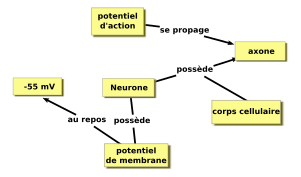
\includegraphics[width=\linewidth]{study5-conceptmap.png}
        \end{subfigure} \\
        \begin{subfigure}{.7\textwidth}
            \includegraphics[width=\linewidth]{study5-kat.png}
        \end{subfigure}
        \caption{Screenshot of the KAT condition during the concept-map building
        phase.}
        \label{study5:kat}
\end{figure*}

\subsubsection*{Subjects}
%ANON
%Sixty-four first year EPFL students (46 men, 18 women, mean age: 21.2)
Sixty-four first year students (46 men, 18 women, mean age: 21.2)
participated to the study. They were randomly assigned to conditions and
did not know each other before. Like in Study 4, students from Life Science
faculty were excluded.

\subsubsection*{Variables}

The participants of the experimental condition group were provided with the
Knowledge Awareness Tool on the bottom part of the screen
(Fig.~\ref{study5:kat}): each line represents the score obtained by the partner
at the pre-test for a chapter. Participants did not see their own score, but they
usually started their discussion by exchanging this information.

\subsubsection*{Results}

\paragraph{Grounding criterion} A linear regression revealed a positive relation
between \gModel{A}{B} and the learning gain of the pair $\{A, B\}$ (calculated
as the average of the individual learning gains): $\beta= 0.401, p < 0.001, r2adj.
= 0.15$, large effect. This relationship was not significant in the previous
experiment which as been conducted with the same task (using the same task
should produce the same grounding criterion). This is probably due to the fact that
\gModel{A}{B} was influenced by the KAT.

\paragraph{Study-specific questions} The $t$-test reported a significant
difference between the KAT condition participants ($M = 13.4\%$) and the control
group $M = 3.6\%$ [$t(1, 60) = 2.73, p < 0.01$, Cohen's $d = 0.7$, medium to large
effect]: providing learners with cues about the prior-knowledge of their partner
enhances their collaborative learning. As a treatment check, we found a positive
and significant correlation between the amount of gazes on KAT (using eye
tracking devices) and the learning gains ($r(22) = 0.54, p = 0.01$). A detailed
analysis revealed that the participants look at KAT to assess their peer's credibility
when he/she provided new information. 

The KAT has a significant effect on \gModel{A}{B}: peers more accurately
estimated their partners knowledge ($M = 1.11$) than those in the control
condition $M = 0.98$ [$t(1, 60) = 3.19, p < 0.01$, Cohen's $d = 0.83$, large
effect]. This is a trivial result since the KAT provided them with an initial
\gmodel{A}{B}. However, the participants have to predict the post-test score while the
KAT informed them about the pre-test score. Actually, pairs in the KAT condition
produced significantly more instances of 3 interesting categories of
interactions: (1) utterances asking about the other's knowledge such as ``Did
you understand how transmission works?'' (2) utterances describing one's own
knowledge (\gmodel{A}{A}) such as ``I don't remember the Ranvier's thing...''
and (3) elaborated utterances with rich contents. These three categories provide
different account of \gModel{A}{B}: (1) as an effect of \A's effort to model
\B  ($\mathcal{H}_{1}$), (2) as \B's effort to give cues to \A about his own
knowledge ($\mathcal{H}_{2}$) and (3) as an effect of the quality of
interaction ($\mathcal{H}_{3}$) .

We examined \gModel{A}{B} as potentially mediating the effect of the KAT factor
on the relative learning gain. A linear regression confirmed that \gModel{A}{B}
was significantly related to the KAT-factor ($\beta= 0.381, p < 0.01, r2 = 0.15$).
The KAT-factor was also significantly and positively related to the RLG ($\beta=
.332, p < 0.01, r2 = 0.11$). We then tested the relation between the independent
variable (KAT) and the dependent variable (gains) when controlling for the
mediating variable (\gModel{A}{B}). A multiple regression showed that the
KAT-factor was no longer a significant predictor ($\beta= 0.210; p = ns$) whereas
the \gModel{A}{B} was still a significant predictor ($\beta= 0.32, p < 0.01$).
Thus, it can be concluded that \gModel{A}{B} mediated the KAT-factor's effect on
the learners' RLG. The Sobel significance test for indirect effects was
significant [$z = 1.99, p < 0.05$]. 

\paragraph{Symmetry question} We did not find an intra-pair correlation ($ICC =
0.05, ns$), which does not support $\mathcal{H}_{2}$ and $\mathcal{H}_{3}$. In
addition, the KAT supports the processing of modelling at the first level
($\mathcal{H}_{1}$) and not at the second level ($\mathcal{H}_{2}$). Hence the
fact that the KAT enhances  \gModel{A}{B}  brings additional supports to
$\mathcal{H}_{1}$. However, the analysis of verbal interactions find elements
that actually supports the three hypotheses.

%\paragraph{Rectangle question} $\Delta_4$: the correlation between \gmodel{A}{A} and \gmodel{A}{B} is
%\fixme{???  MIRWEIS A FAIRE}.

\subsubsection*{Discussion}

Despite the fact that the learning task was the same as in study 4, the
conditions of collaboration (viewing multiple maps or not) and the conditions
(scripted or not, awareness tool or not) probably explain differences in terms
of mutual modelling.

\section{Synthesis}

We found a symmetry of the mutual models on 4 studies out of 5. In study 4, this
only applies to the control group (having read the same text before), which
corresponds to the situation of the 3 first studies. Evidencing this symmetry
constitutes \textit{per se} an interesting result as we are not aware of earlier
studies who have established this relationship.
Still, the symmetry alone does not allow to discriminate $\mathcal{H}_{2}$ from
$\mathcal{H}_{3}$. The second hypothesis (\ie mutual modelling is primarily
supported by the capacity of the modellee to help the modellers to form a
correct image of herself), is questioned by study 3 where \C could be modelled
accurately by \A and not accurately by \B. The same hypothesis is however
supported by the results of study 2, and indirectly by study 4.

This does not rule out entirely $\mathcal{H}_{1}$ (\ie partner modelling is
primarily a individual skill) either: even where we found significant
correlations, they were all below 0.50, not around 0.90.  Hence, even if the
quality of the social interaction matters, there is obviously a large part of
individual variance within teams.

In other words, these studies do not conclude that one hypothesis is right and the
others are wrong, and this is indeed the main contribution of this article. We
started from the idea that partner modelling is essentially an individual skill
and that we would therefore improve the quality of collaboration by providing 
awareness tools, as those tools would act as a kind of prosthesis for partner
modelling. The role and importance of this individual skill cannot be discarded:
everyone has experienced the pleasure of interacting with colleagues who answer precisely to the question
we asked them and even guess the reason why we asked this question. Conversely,
everyone also experienced the frustration of someone referring about a third
person by his name, say Mike Smith, while knowing perfectly that there is no
chance that we know this Mike Smith. In fact, the role of this individual skill is
not denied by our studies; the novelty of this paper is to show, thanks to
symmetry values, that individual skills only account for a part of the accuracy
in mutual modelling.

We acknowledge that the difference between these hypotheses is rather
theoretical since the  process of modelling one's partner $\mathcal{H}_{1}$ and
the process of helping one's partner to model oneself $\mathcal{H}_{2}$ are
mediated by verbal interactions in the team. One could hardly imagine someone
managing a very accurate modelling despite the very bad quality of interactions.
There is a bidirectional causal link between the accuracy of mutual modelling
and the quality of the interactions. This rather artificial distinction does
however participate to the more fundamental discussion of the role of individual
and social mechanisms in human cognition. In the field of social cognition, it
is a common place to state that ``the whole is greater than the sum of the
parts''.  This refers to the emergence of team properties than cannot be reduced
to the set of individual contributions. Our paper illustrates this emergence by
showing the symmetry of mutual modelling.


These conclusions must be presented with multiple disclaimers. First, they
heavily rely on correlations; hence we cannot identify causal links. Second, we
faced hard methodological issues. Providing learners with on-task questionnaires
introduces a bias: they will pay more attention to their partners in the
remaining time. Providing them with ``after-task'' questionnaires implies
mnemonic and rationalization biases. The nature of mutual modelling implies
methodological challenges that call for new measurement methods. We have
promising results for using eye tracking methods to address this challenge.
Third, our results emerge from a post-hoc reinterpretation of studies that
addressed different research questions (media richness, awareness tools,
scripts,...). This diversity makes our results difficult to integrate, partly
contradictory. Nonetheless, this diversity also incidentally provides some
generalizability: mutual modelling has been investigated in different contexts
(virtual space versus real space), with different groups sizes (pairs and
triads) and different tasks.

Finally, let us repeat that the expressions we used, such as \gmodel{A}{B}, do
not imply we have a mechanical view of modelling. It's just a language for
referring to different components of modelling each other in teams.  This simple
notation emerged from the need to compare five mutual modelling studies. It
could however pave the road for elaborating a systematic agenda for research on
mutual modelling.

\begin{acknowledgements}

%ANON
%The experiments were developed with the help of Mirweis Sangin, René Glaus,
%Patrick Jermann,  Fabien Girardin, Marc-Antoine Nüssli, Thomas Werhle, Yvan
%Bourquin and Jeremy Goslin.  We also thank Kshitij Sharma and {\L}ukasz
%Kidzi\'nski for their help with data analysis. The main funding has been
%provided from a NSF Grant grant \#102511-106940.

\textit{Removed for blind review.}

\end{acknowledgements}

%%%%%%%%%%%%%%%%%%%%%%%%%%%%%%%%%%%%%%%%%%%%%%%%%%%%%%%%%%%%%%%%%%%%%%%%%%%%%%%
\bibliographystyle{spbasic}
\bibliography{biblio}



\end{document}

